El módulo \texttt{metro.py} contiene los siguientes objetos:
\begin{itemize}[leftmargin=0pt]
  \item el diccionario \verb!estaciones!,
    que asocia a cada línea del metro
    (\verb!'1'!, \verb!'2!', \verb!'4'!, \verb!'4A'!, \verb!'5'!)
    la lista de sus estaciones
    en el orden de su recorrido;
  \item el diccionario \verb!coordenadas!,
    que asocia a cada estación de metro
    una tupla con sus coordenadas geográficas
    (latitud y longitud).
\end{itemize}

\begin{enumerate}[leftmargin=0pt,label=\emph{\alph*})]
  \item
    Escriba un programa llamado \texttt{combinacion.py}
    que imprima \textbf{todas} las estaciones de combinación
    siguiendo el siguiente formato:
    \lstinputlisting[
      linerange=SALIDA-FIN\ SALIDA,
      frame=single
    ]{metro/combinacion.py}

  \item
    Escriba un programa llamado \texttt{extremas.py}
    que muestre cuáles son las estaciones que están
    más al norte, al sur, al este y al oeste
    de toda la red:
    \lstinputlisting[
      linerange=SALIDA-FIN\ SALIDA,
      frame=single
    ]{metro/extremas.py}

  \newpage
  \item
    Escriba las siguientes funciones:
    \lstinputlisting{metro/casos.txt}

  \newpage
  \item
    Escriba un programa llamado \verb!dibujar_red.py!
    que haga que la tortuga dibuje la red del metro:

    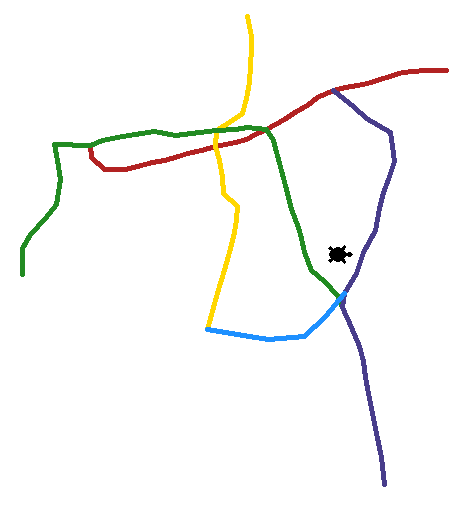
\includegraphics[height=250px]{metro/red1}

    Las funciones del módulo \texttt{turtle}
    que le serán útiles son:
    \texttt{up()},
    \texttt{down()},
    \texttt{goto(x, y)} y
    \texttt{color('nombre del color')}.

  \newpage
  \item
    Modifique su programa para que la tortuga
    dibuje también las estaciones:

    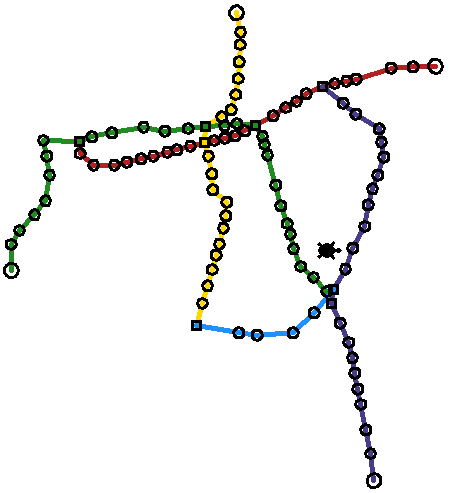
\includegraphics[height=250px]{metro/red2}

    Utilice para esto las funciones provistas
    por el módulo \texttt{figuras.py}.
    Las estaciones de combinación deben ser representadas
    con un cuadrado
    y las estaciones terminales
    con un círculo más grande.

  \newpage
  \item
    Modifique su programa para que la tortuga
    escriba los nombres de las estaciones
    de las líneas 2 y 4:

    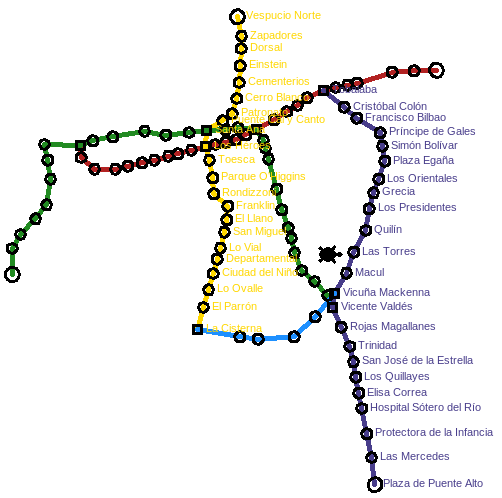
\includegraphics[height=250px]{metro/red3}

    Utilice para esto la función \lstinline!write('Texto')!
    provista por el módulo \verb!turtle!.

\end{enumerate}
